\chapter{Subdivision Plugin}

Die Hauptfunktionalität des Programms SubVis wird ebenfalls in einem Plugin bereitgestellt. 
Dieses erlaubt die Anwendung verschiedener Unterteilungsalgorithmen und das Rendering deren Limes-Flächen.

\begin{figure}
  \centering
  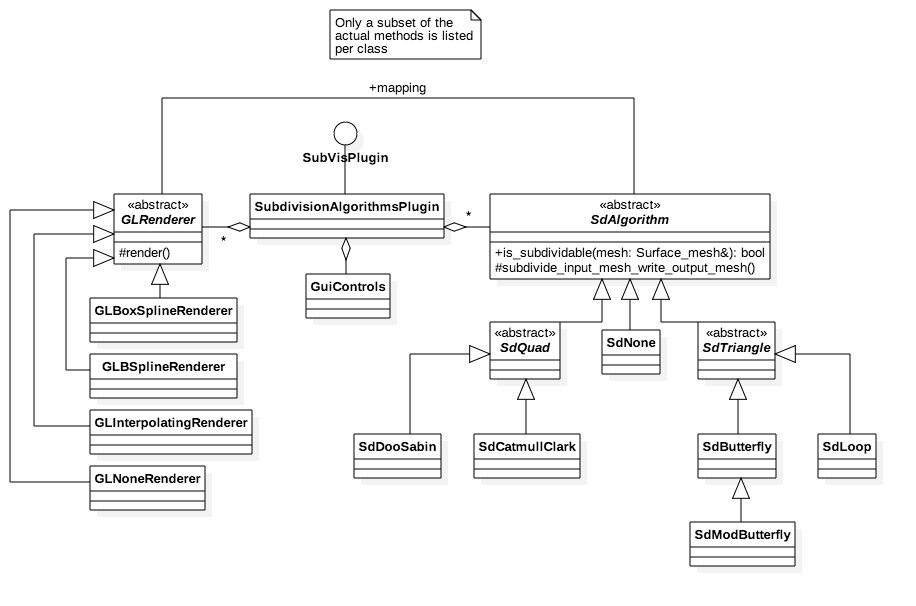
\includegraphics[width=\textwidth]{content/media/subvis_architektur_plugin_subdivision.png}
  \caption{Architektur des Subdivision-Plugins}
  \label{fig:subvis_architektur_plugin_subdivision}
\end{figure}

\autoref{fig:subvis_architektur_plugin_subdivision} gibt einen Überblick über die Architektur.
Die Hauptklasse ist \emph{SubdivisionAlgorithmsPlugin} welche auch die SubVisPlugin  Schnittstelle implementiert.
Die GUI, das Rendering und die Algorithmen wurden in jeweils eigene Klassen ausgelagert.

\section{GUI}

\begin{figure}
  \centering
  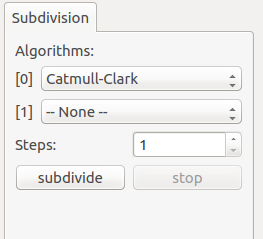
\includegraphics[width=0.3\textwidth]{content/media/subvis_plugin.png}
  \caption{GUI-Elemente des Plugins}
  \label{fig:subivs_plugin_gui}
\end{figure}

Die GUI besteht aus zwei Auswahllisten für den Algorithmus pro Polygonnetz, einer Einstellung für die Anzahl an Unterteilungsschritten und einem Start bzw. Stop Button (siehe \autoref{fig:subivs_plugin_gui}).

\section{Rendering}

Jeder Renderer erweitert die abstrakte Klasse \emph{GLRenderer}. 
Diese ruft mittels Template-Pattern eine Methode \emph{render} ihrer Unterklasse auf, um den Rendervorgang zu starten.
Bei Veränderungen der Model-Komponente wird das Polygonnetz kopiert, damit Unterklassen das Polygonnetz verändern können.

\subsection{Kontrollnetz}
..


\subsection{Limes-Fläche}
..

\section{Algorithmen}

Die Algorithmen werden über die abstrakte Klasse \emph{SdAlgorithm} zusammengefasst. 
Diese ermöglicht es, der GUI abzufragen, ob ein bestimmtes Polygonnetz von diesem Algorithmus unterteilt werden kann oder nicht, was sich in der Auswahlmöglichkeit der GUI niederschlägt.
Außerdem implementiert die Klasse die Verwaltung der Polygonnetze und ein Thread-basiertes unterteilen. 
Somit müssen die konkreten Klassen der Algorithmen lediglich eine Methode überschreiben und sich nur auf die korrekte Implementierung fokussieren.
Es werden vor jedem Aufruf der Unterklasse die Variablen \emph{input\_mesh} und \emph{output\_mesh} entsprechend initialisiert.
Die Unterklassen müssen dann pro Aufruf von \emph{subdivide\_input\_mesh\_write\_output\_mesh} das Eingangsnetz lesen und das Ergebnis in der Variable output\_mesh speichern.

\begin{lstlisting}[style=myCppStyle, caption={Signatur der Unterteilungsfunktion}, label=lst:subdiv_threaded]
void subdivide_threaded(const Surface_mesh& mesh, 
std::function<void(std::unique_ptr<Surface_mesh>)> callback, 
const int steps = 1);
\end{lstlisting}

Das Thread-basierte Rendering ist über einen Callback-Mechanismus implementiert (vgl. \autoref{lst:subdiv_threaded}), welcher garantiert, dass die Callback-Funktion auf dem UI-Thread ausgeführt wird.
Die Funktion subdivide\_threaded ruft eine Worker-Funktion mittels QtConcurrent::run auf, welche in einer Schleife die konkrete Implementierung der Unterteilung ausführt.
Die Worker-Funktion sendet am Ende ihrer Ausführung ein Signal \emph{finished} aus.
Dieses wiederum wird von der Klasse empfangen und in einen Aufruf der Callback-Funktion umgesetzt.
Durch Verwendung des Signal-Slot Konzepts ist garantiert, dass der Slot und somit der Callback auf dem UI-Thread ausgeführt wird.
Der implementierte Callback-Mechanismus macht somit das Threading wesentlich einfacher und benötigt keine Synchronisierungsmechanismen.

Als konkreter Callback wird eine Funktion verwendet, die bei Beendigung das Ergebnis in die Model-Komponente lädt (was ein Neuzeichnen des Polygonnetzes zur Folge hat).

\subsection{Catmull Clark}
..
..



















